% TU Delft Beamer template
% Author: Maarten Abbink
% Delft University of Technology
% March 2014
% Version 2.0
% Based on original version 1.0 of Carl Schneider
\documentclass{beamer}
\usepackage[english]{babel}
\usepackage{calc}
\usepackage[absolute,overlay]{textpos}
\mode<presentation>{\usetheme{tud}}

\title[Beamer Sample]{Sample presentation using Beamer}
%\subtitle
\institute[TU Delft]{Delft University of Technology}
\author{Maarten Abbink}
\date{\today}

% Insert frame before each subsection (requires 2 latex runs)
\AtBeginSubsection[] {
	\begin{frame}<beamer>\frametitle{\titleSubsec}
		\tableofcontents[currentsection,currentsubsection]  % Generation of the Table of Contents
	\end{frame}
}
% Define the title of each inserted pre-subsection frame
\newcommand*\titleSubsec{Next Subsection}
% Define the title of the "Table of Contents" frame
\newcommand*\titleTOC{Outline}

% define a symbol which can be removed if you don't need it
\newcommand{\field}[1]{\mathbb{#1}}
\newcommand{\Zset}{\field{Z}}

\begin{document}

{
% remove the next line if you don't want a background image
\usebackgroundtemplate{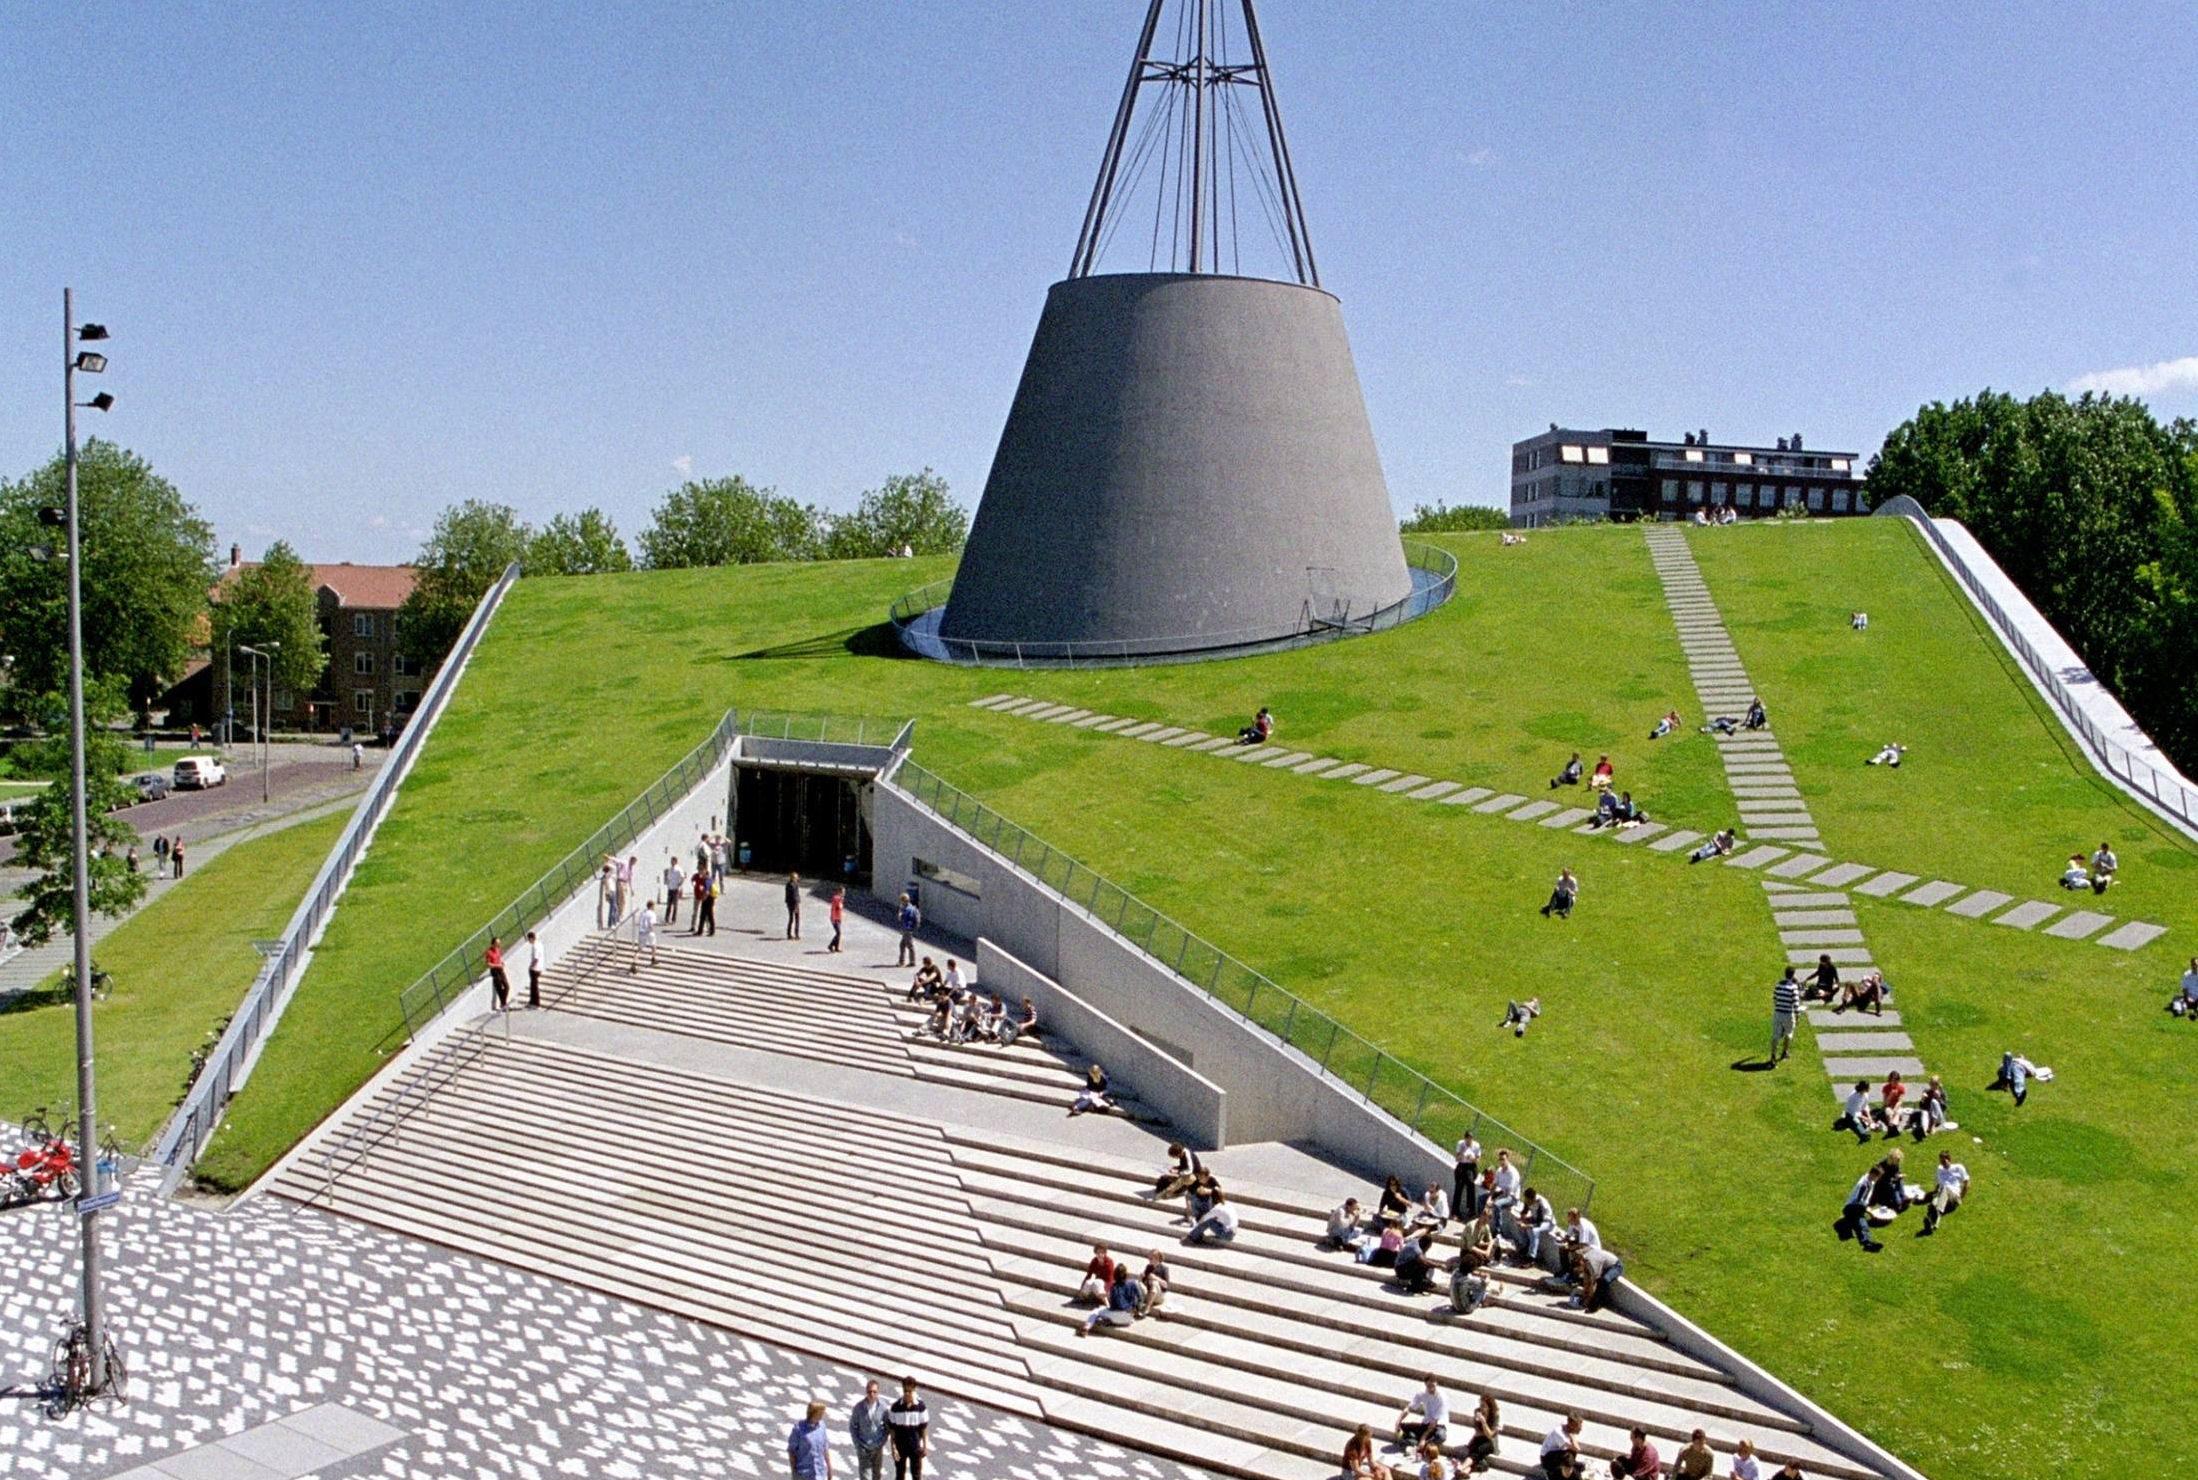
\includegraphics[width=\paperwidth,height=\paperheight]{images/background-titlepage.jpg}}%
\setbeamertemplate{footline}{\usebeamertemplate*{minimal footline}}
\frame{\titlepage}
}

{\setbeamertemplate{footline}{\usebeamertemplate*{minimal footline}}
\begin{frame}\frametitle{\titleTOC}
	\tableofcontents
\end{frame}
}

\section{First Section}
\subsection{Section 1 - Subsection 1}

\begin{frame}\frametitle{Section 1 - Subsection 1 - Page 1}
	\begin{example}
		\begin{minipage}{0.6\textwidth}
			% insert picture (pdf file)
			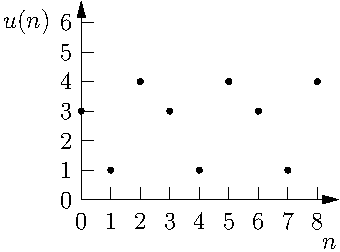
\includegraphics{images/ex1_periodic_number.pdf}
		\end{minipage}
		\centering{$u(n)=[3,1,4]_n$}
	\end{example}
\end{frame}

\begin{frame}\frametitle{Section 1 - Subsection 1 - Page 2}
	\begin{definition}
		Let $n$ be a discrete variable, i.e. $n\in\Zset$.
		A 1-dimensional periodic number is a function that depends periodically on $n$.
		$$
		u(n)=
		[u_0,u_1,\ldots,u_{d-1}]_n=
		\begin{cases}
			u_0 & \mbox{ if $n\equiv 0 \pmod d$} \\
			u_1 & \mbox{ if $n\equiv 1 \pmod d$} \\
			\vdots \\
			u_{d-1} & \mbox{ if $n\equiv d-1 \pmod d$}
		\end{cases}
		$$
		$d$ is called the period.
	\end{definition}
\end{frame}

\begin{frame}\frametitle{Section 1 - Subsection 1 - Page 3}
	%this is too big.
	\begin{example}
		\centering
		{
		$$
		\begin{array}{rcl}
			f(n)
			&=&
			-\left[\frac{1}{2},\frac{1}{3}\right]_n n^2
			+3n-[1,2]_n
			\\
			&=&
			\begin{cases}
				-\frac{1}{3} n^2 +3n-2
				& \text{ if $n\equiv 0 \pmod 2$} \\
				-\frac{1}{2} n^2 +3n-1
				& \text{ if $n\equiv 1 \pmod 2$}
			\end{cases}
			% &=&
			% -\frac{n^2}{2}+3n-1
			% -\left\{ \frac{n}{2} \right\}
			% \left( \frac{2}{3}n^2+2
			% \right)
		\end{array}
		$$
		\begin{minipage}{0.4\textwidth}
			% insert picture (pdf file)
			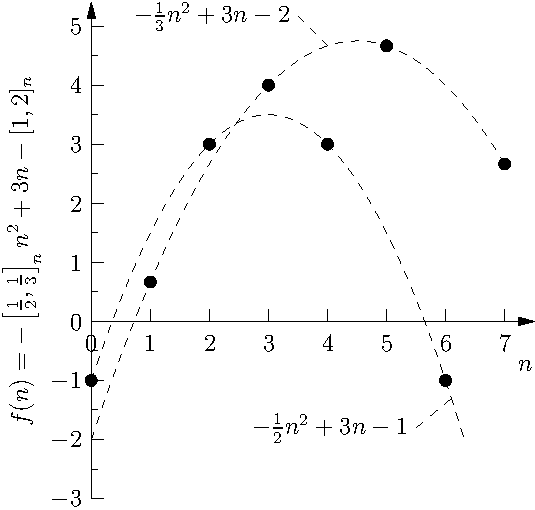
\includegraphics[width=\textwidth]{images/ex2_quasi_polynomial.pdf}
		\end{minipage}
		}
	\end{example}
\end{frame}

\begin{frame}\frametitle{Section 1 - Subsection 1 - Page 4}
	% Show first part of the screen highlighted
	\begin{definition}
		A polynomial in a variable $x$ is a linear combination of powers of $x$:
		$$
		f(x)=\sum_{i=0}^g c_i x^i
		$$
	\end{definition}
	\pause
	
	% Show second part of the screen highlighted
	\begin{definition}
		A quasi-polynomial in a variable $x$ is a polynomial expression with periodic numbers as coefficients:
		$$
		f(n)=\sum_{i=0}^g u_i(n) n^i
		$$
		with $u_i(n)$ periodic numbers.
	\end{definition}
\end{frame}

\subsection{Section 1 - Subsection 2}

\begin{frame}\frametitle{Section 1 - Subsection 2 - Page 1}
	\begin{example}
		\begin{columns}
			\column{0.40\textwidth}
			\centering
			\includegraphics<1>[width=\textwidth]{images/ex3a_pp.pdf}
			\includegraphics<2>[width=\textwidth]{images/ex3b_pp.pdf}
			\includegraphics<3>[width=\textwidth]{images/ex3c_pp.pdf}
			\includegraphics<4->[width=\textwidth]{images/ex3d_pp.pdf}
			{ \textbf{\small{{$x+y\le p$}}}}
			\column{0.1\textwidth}
			
			\begin{tabular}{c c}
				$p$ & $f(p)$ \\ \hline
				3 & 5 \\
				\pause
				4 & 8 \\
				\pause
				5 & 10 \\
				\pause
				6 & 13 \\
			\end{tabular}
			
			\column{0.3\textwidth}
			\pause
			$$
			\frac{5}{2}p+\left[-2,\frac{-5}{2} \right]_p
			$$
		\end{columns}
	\end{example}
\end{frame}

\begin{frame}\frametitle{Section 1 - Subsection 2 - Page 2}
	\begin{itemize}
		\item <1-> The number of integer points in a \alert{parametric polytope} $P_{{p}}$ of dimension $n$ is expressed as a piecewise a quasi-polynomial of degree $n$ in ${p}$ (Clauss and Loechner).
		
		\item <2->
		More general \alert{polyhedral counting problems}:\\
		Systems of linear inequalities combined with $\lor, \land, \neg, \forall,$ or $\exists$ (Presburger formulas).
		\item <3->
		Many problems in \alert{static program analysis} can be expressed as polyhedral counting problems.
	\end{itemize}
\end{frame}

\subsection{Section 1 - Subsection 3}

\begin{frame}\frametitle{Section 1 - Subsection 3 - Page 1}
	% Just an example
	A picture made with the package TiKz\\
	\begin{example}
		\centering
		%Number of live elements = quasi-polynomial\\
		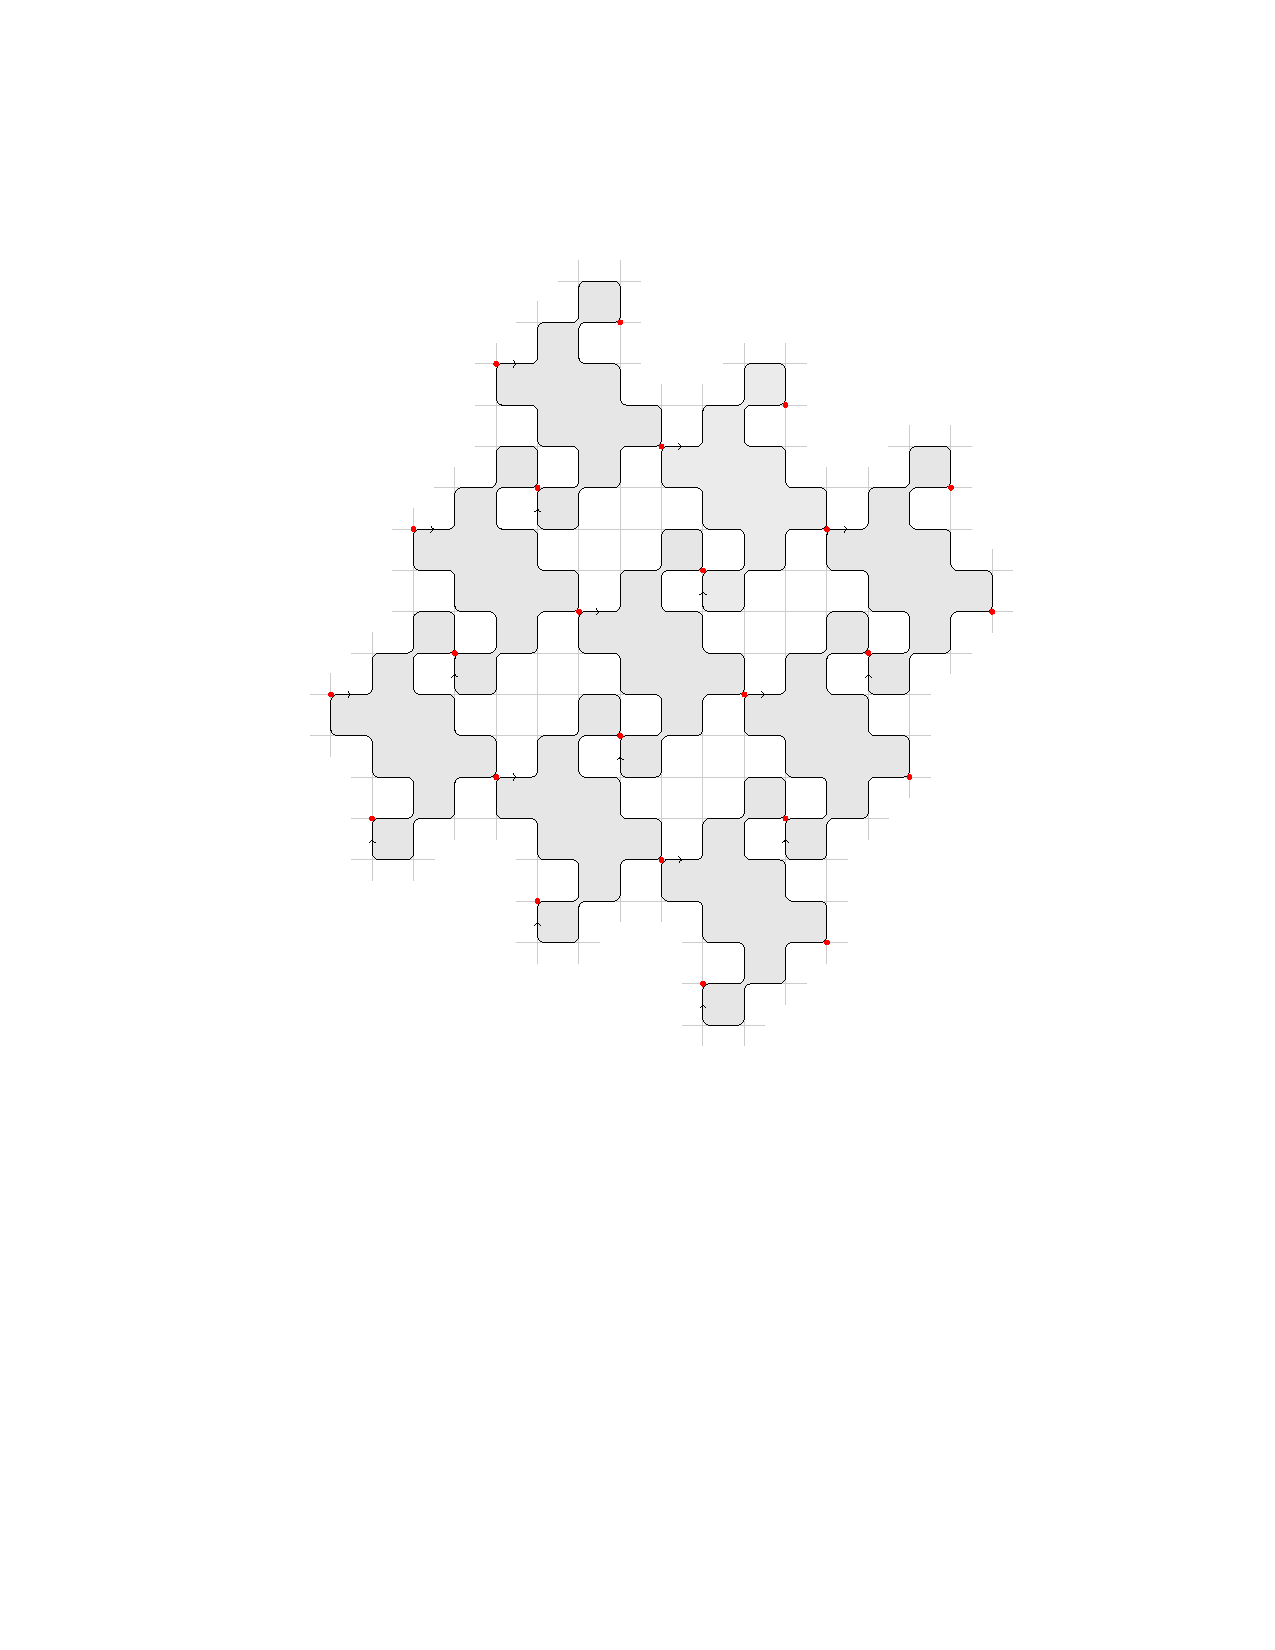
\includegraphics[width=5cm]{images/abadab-anti-theta-01.pdf}
		%$\Downarrow$ \\
		%Memory usage = maximum over all execution points
	\end{example}
\end{frame}

\section{Second Section}

\subsection{Section 2 - Subsection 1}

\begin{frame}\frametitle{Section 2 - subsection 1 - page 1}
	\begin{alertblock}{Alertblock}
		This page gives an example with numbered bullets (enumerate)\\
		in an "Example" window:\\
	\end{alertblock}
	
	\begin{example}
		Discrete domain $\Rightarrow$ evaluate in each point\\
		Not possible for\\
		\begin{enumerate}
			\item <1-> parametric domains
			\item <2-> large domains (NP-complete)
		\end{enumerate}
	\end{example}
\end{frame}

\subsection[]{Section 2 - Last Subsection}

\begin{frame}\frametitle{Last Page}
	\begin{block}{Summary}
		\centering{End of the beamer demo\\
		with a \emph{tidy} TU~Delft lay-out.\\
		Thank you!}
	\end{block}
\end{frame}

\end{document}
